% Modelo cinemático continuo de tracción diferencial (vista superior).
% Notación de la subsección "Modelo de Tracción Diferencial" (fundamentos_teoricos.tex).
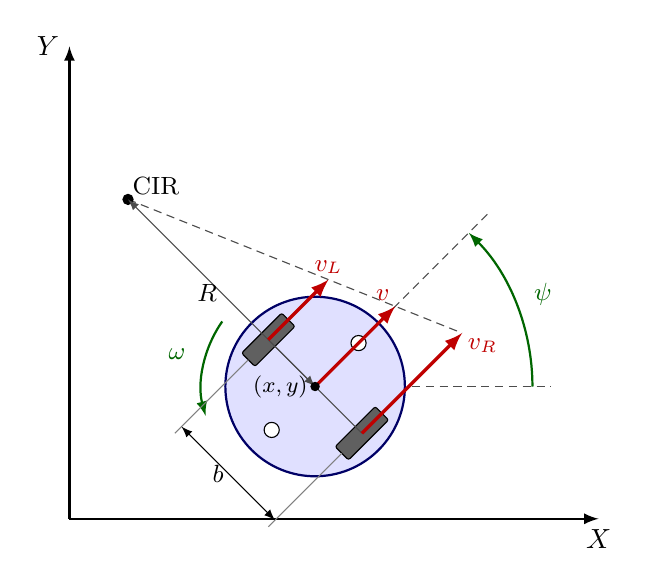
\begin{tikzpicture}[scale=1.2, >=latex,
        cuerpo/.style={fill=blue!12, draw=blue!40!black, thick},
        rueda/.style={fill=gray!75!black, draw=black, rounded corners=0.8pt},
        loca/.style={fill=white, draw=black},
        veloc/.style={->, very thick, red!75!black},
        angulo/.style={->, thick, green!40!black},
        guia/.style={gray!60!black, densely dashed},
        cota/.style={<->, thin},
        etiq/.style={font=\small, inner sep=1.5pt},
        ejes/.style={->, thick}]
\def\psiD{45}      % rumbo psi (grados)
\def\bb{0.7}       % semidistancia entre ruedas, b/2
\def\vL{0.9}       % longitud de la flecha v_L
\def\vR{1.5}       % longitud de la flecha v_R
% CIR sobre el eje de las ruedas: R = (b/2)(vR+vL)/(vR-vL)
\pgfmathsetmacro{\RD}{\bb*(\vR+\vL)/(\vR-\vL)}
\pgfmathsetmacro{\vD}{(\vR+\vL)/2}
% Ejes globales
\draw[ejes] (0,0) -- (5.6,0) node[below] {$X$};
\draw[ejes] (0,0) -- (0,5.0) node[left] {$Y$};
% Referencia horizontal para el rumbo
\draw[guia] (2.6,1.4) -- (5.1,1.4);
\draw[angulo] (2.6,1.4) ++(0:2.3) arc (0:\psiD:2.3);
\path (2.6,1.4) ++(22:2.6) node[etiq, text=green!40!black] {$\psi$};
\begin{scope}[shift={(2.6,1.4)}, rotate=\psiD]
    % Eje longitudinal del robot
    \draw[guia] (0,0) -- (2.6,0);
    % Chasis y ruedas
    \draw[cuerpo] (0,0) circle (0.95);
    \draw[rueda] (-0.3,\bb-0.1) rectangle (0.3,\bb+0.1);
    \draw[rueda] (-0.3,-\bb-0.1) rectangle (0.3,-\bb+0.1);
    \draw[loca] (0.65,0) circle (0.08);
    \draw[loca] (-0.65,0) circle (0.08);
    \draw[thin, black!70] (0,-\bb) -- (0,\bb);
    % Distribución lineal de velocidades respecto al CIR
    \draw[guia] (0,\RD) -- (\vR,-\bb);
    \fill[black] (0,\RD) circle (0.06)
        node[etiq, above right] {CIR};
    \draw[cota, gray!60!black] (0,0) -- (0,\RD)
        node[etiq, midway, left, text=black] {$R$};
    % Velocidades de las ruedas y del punto medio del eje
    \draw[veloc] (0,\bb) -- (\vL,\bb)
        node[etiq, above, text=red!75!black] {$v_L$};
    \draw[veloc] (0,-\bb) -- (\vR,-\bb)
        node[etiq, below right, text=red!75!black] {$v_R$};
    \draw[veloc] (0,0) -- (\vD,0)
        node[etiq, above left, text=red!75!black] {$v$};
    % Velocidad angular del chasis
    \draw[angulo] (100:1.2) arc (100:150:1.2);
    \node[etiq, text=green!40!black] at (122:1.5) {$\omega$};
    % Distancia entre ruedas
    \draw[thin, gray] (-0.3,\bb) -- (-1.4,\bb) (-0.3,-\bb) -- (-1.4,-\bb);
    \draw[cota] (-1.3,-\bb) -- (-1.3,\bb)
        node[etiq, midway, left] {$b$};
    % Punto de referencia (x, y)
    \fill[black] (0,0) circle (0.05);
\end{scope}
\node[etiq, left=1pt, font=\footnotesize] at (2.6,1.4) {$(x,y)$};
\end{tikzpicture}
